\chapter{Consideraciones sobre la implementación}

\section{Visión general}

En capítulo se hace referencia a las consideraciones sobre la implementación del proyecto, es decir, a los aspectos más significativos a la hora de codificar el sistema y sus funcionalidades. Se explicarán algunos de los pasos que se han dado a la hora de programar el sistema entero para que así, en caso de ser necesaria una expansión o revisión del proyecto, requiera emplear el menor esfuerzo posible a la hora de comprender lo que está desarrollado.

\section{Entorno de desarrollo}

Las herramientas que se han utilizado para facilitar la estructuración y desarrollo del proyecto han sido las siguientes:

\subsection{Git}

Git\cite{Git} es un software de control de versiones gratuito de código abierto diseñado por Linus Torvalds pensando en la eficiencia y la confiabilidad del mantenimiento de versiones de aplicaciones, más aún cuando estas tienen un gran número de archivos de código fuente, tanto de pequeños proyectos particulares como proyectos de grandes organizaciones. 

\begin{figure}[!htp]
	 \centering
	 
\includegraphics[scale=0.8]{fig/git_logo}
	 \caption{Logotipo de Git}
\end{figure}

Al principio, Git se pensó como un motor de bajo nivel sobre el cual otros pudieran escribir interfaces de usuario. Sin embargo, Git se ha convertido desde entonces en un sistema de control de versiones con funcionalidad plena. Hay algunos proyectos de mucha relevancia que ya usan Git, en particular, el grupo de programación del núcleo Linux.

Por otra parte la curva de aprendizaje de este sistema es relativamente baja, contando con una excelente documentación, pero más importante aún, al ser usado por muchos desarrolladores ha generado una comunidad de usuarios dispuesta a resolver cualquier problema.

En lo que respecta a este proyecto, se ha decidido usar los repositorios gratuitos ofrecidos por GitHub\cite{Github} para mantener el control de versiones de todo el código. El hecho de disponer una cuenta de estudiantes ha permitido hacer privados los repositorios para el almacenamiento seguro en la nube de forma gratuita.

\subsection{Sublime Text 2}

Sublime Text\cite{SublimeText} es un editor de texto y código fuente, escrito en C++ y Python, multiplataforma con una clara e intuitiva interfaz desarrollado especialmente para programadores que presenta varias características para mejorar la eficiencia de los desarrolladores. Entre estas ventajas cabe destacar el auto-completado, la capacidad de resaltar las expresiones propias de numerosos lenguajes, tales como \acrlong{js}, Python, \acrshort{html}, \acrshort{css}, visualizar más de un fichero a la vez por pantalla, etc. 

\begin{figure}[!htp]
	 \centering
	 
\includegraphics[scale=0.2]{fig/sublime_text_logo}
	 \caption{Logotipo de Sublime Text}
\end{figure}

Además, Sublime Text incluye una \acrshort{api} que permite desarrollar extensiones para dar soporte a más lenguajes o añadir nuevas herramientas y funcionalidades que hagan más sencilla la tarea de programar las aplicaciones.

\subsection{Google Chrome}

Google Chrome\cite{Chrome} es un navegador web desarrollado por Google\cite{Google} que incorpora herramientas para facilitar el desarrollo web para las distintas plataformas de sobremesa, tabletas y móviles.

\begin{figure}[!htp]
	 \centering
	 
\includegraphics[scale=0.4]{fig/chrome}
	 \caption{Logotipo de Google Chrome}
\end{figure}

Entre las características para el desarrollo web que dispone se ha utilizado el modo dispositivo y emulación móvil\cite{DeviceMode} que ha facilitado realizar las siguientes tareas:

\begin{itemize}
	\item Comprobar el diseño responsivo de la aplicación web en distintos tamaños de pantallas y resoluciones.
	\item Visualizar e inspeccionar el \acrshort{css} y las \textit{media queries}.
	\item Simular los eventos de entrada del dispositivo como las pulsaciones y la orientación de la pantalla.
\end{itemize}

En la siguiente figura (\ref{fig:google_device}) puede verse un ejemplo de la vista del entorno de desarrollo en Google Chrome.

\begin{figure}[!htp]
	 \centering
	 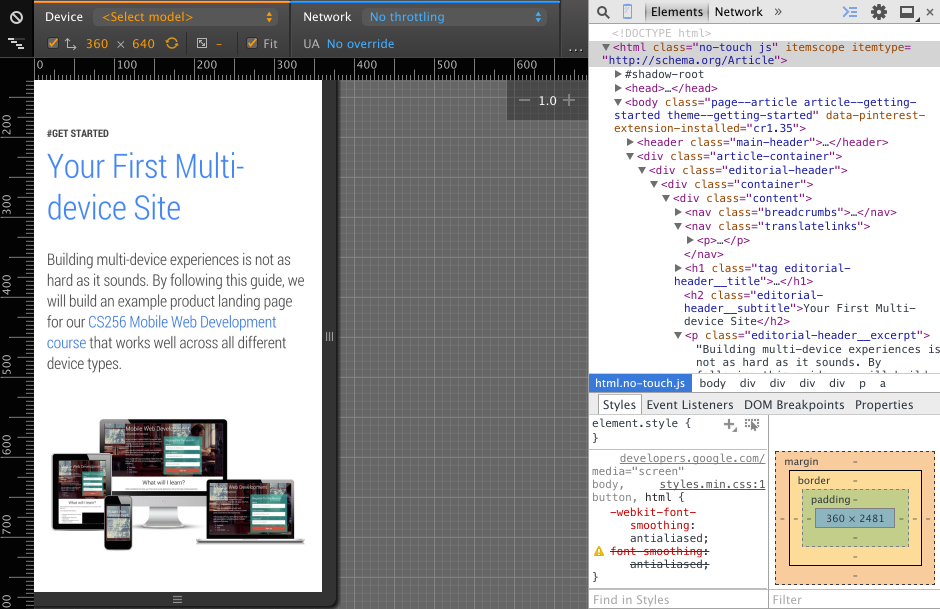
\includegraphics[scale=0.44]{fig/device_mode}
	 \caption{Modo dispositivo de Google Chrome}
	 \label{fig:google_device}
\end{figure}

\section{Calculo de la fecha de moficiación para OAI-PMH}

\begin{figure}[!htbp]
	\centering
	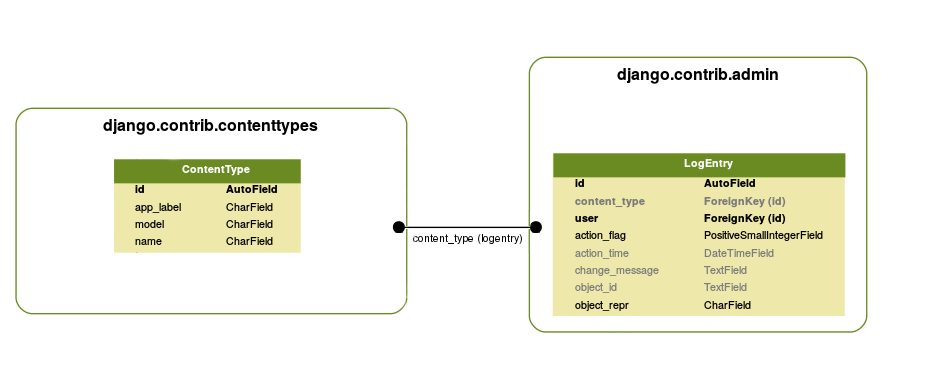
\includegraphics[scale=0.45]{fig/dbmodel/django_log}
	\caption{Modelo de datos relacional del sistema de ``logs'' de Django}
	\label{fig:logsmodel}
\end{figure}